\documentclass{report}
\usepackage{tikz}
\usepackage{pdfpages}
\usetikzlibrary{matrix,calc}

\usepackage{amssymb}
\usepackage{amsmath}
\usepackage{centernot}
\usepackage{scalerel}
\usepackage{stackengine}
\usepackage{xcolor}
\usepackage{circuitikz}
\usepackage{graphicx}
\usepackage{tkz-graph} % for drawing vector graphs
%\usepackage[margin=0.5in]{geometry}
\usepackage[top=1in,bottom=1in]{geometry}

\newcommand\showdiv[1]{\overline{\smash{\hstretch{.5}{)}\mkern-3.2mu\hstretch{.5}{)}}#1}}
\newcommand\ph[1]{\textcolor{white}{#1}}


\makeatletter
% we use \prefix@<level> only if it is defined
\renewcommand{\@seccntformat}[1]{%
  \ifcsname prefix@#1\endcsname
    \csname prefix@#1\endcsname
  \else
    \csname the#1\endcsname\quad
  \fi}
% define \prefix@section
\newcommand\prefix@section{}
\newcommand\prefix@subsection{}
\makeatother


%isolated term
%#1 - Optional. Space between node and grouping line. Default=0
%#2 - node
%#3 - filling color
\newcommand{\implicantsol}[3][0]{
    \draw[rounded corners=3pt, fill=#3, opacity=0.3] ($(#2.north west)+(135:#1)$) rectangle ($(#2.south east)+(-45:#1)$);
    }


%internal group
%#1 - Optional. Space between node and grouping line. Default=0
%#2 - top left node
%#3 - bottom right node
%#4 - filling color
\newcommand{\implicant}[4][0]{
    \draw[rounded corners=3pt, fill=#4, opacity=0.3] ($(#2.north west)+(135:#1)$) rectangle ($(#3.south east)+(-45:#1)$);
    }

%group lateral borders
%#1 - Optional. Space between node and grouping line. Default=0
%#2 - top left node
%#3 - bottom right node
%#4 - filling color
\newcommand{\implicantcostats}[4][0]{
    \draw[rounded corners=3pt, fill=#4, opacity=0.3] ($(rf.east |- #2.north)+(90:#1)$)-| ($(#2.east)+(0:#1)$) |- ($(rf.east |- #3.south)+(-90:#1)$);
    \draw[rounded corners=3pt, fill=#4, opacity=0.3] ($(cf.west |- #2.north)+(90:#1)$) -| ($(#3.west)+(180:#1)$) |- ($(cf.west |- #3.south)+(-90:#1)$);
}

%group top-bottom borders
%#1 - Optional. Space between node and grouping line. Default=0
%#2 - top left node
%#3 - bottom right node
%#4 - filling color
\newcommand{\implicantdaltbaix}[4][0]{
    \draw[rounded corners=3pt, fill=#4, opacity=0.3] ($(cf.south -| #2.west)+(180:#1)$) |- ($(#2.south)+(-90:#1)$) -| ($(cf.south -| #3.east)+(0:#1)$);
    \draw[rounded corners=3pt, fill=#4, opacity=0.3] ($(rf.north -| #2.west)+(180:#1)$) |- ($(#3.north)+(90:#1)$) -| ($(rf.north -| #3.east)+(0:#1)$);
}

%group corners
%#1 - Optional. Space between node and grouping line. Default=0
%#2 - filling color
\newcommand{\implicantcantons}[2][0]{
    \draw[rounded corners=3pt, opacity=.3] ($(rf.east |- 0.south)+(-90:#1)$) -| ($(0.east |- cf.south)+(0:#1)$);
    \draw[rounded corners=3pt, opacity=.3] ($(rf.east |- 8.north)+(90:#1)$) -| ($(8.east |- rf.north)+(0:#1)$);
    \draw[rounded corners=3pt, opacity=.3] ($(cf.west |- 2.south)+(-90:#1)$) -| ($(2.west |- cf.south)+(180:#1)$);
    \draw[rounded corners=3pt, opacity=.3] ($(cf.west |- 10.north)+(90:#1)$) -| ($(10.west |- rf.north)+(180:#1)$);
    \fill[rounded corners=3pt, fill=#2, opacity=.3] ($(rf.east |- 0.south)+(-90:#1)$) -|  ($(0.east |- cf.south)+(0:#1)$) [sharp corners] ($(rf.east |- 0.south)+(-90:#1)$) |-  ($(0.east |- cf.south)+(0:#1)$) ;
    \fill[rounded corners=3pt, fill=#2, opacity=.3] ($(rf.east |- 8.north)+(90:#1)$) -| ($(8.east |- rf.north)+(0:#1)$) [sharp corners] ($(rf.east |- 8.north)+(90:#1)$) |- ($(8.east |- rf.north)+(0:#1)$) ;
    \fill[rounded corners=3pt, fill=#2, opacity=.3] ($(cf.west |- 2.south)+(-90:#1)$) -| ($(2.west |- cf.south)+(180:#1)$) [sharp corners]($(cf.west |- 2.south)+(-90:#1)$) |- ($(2.west |- cf.south)+(180:#1)$) ;
    \fill[rounded corners=3pt, fill=#2, opacity=.3] ($(cf.west |- 10.north)+(90:#1)$) -| ($(10.west |- rf.north)+(180:#1)$) [sharp corners] ($(cf.west |- 10.north)+(90:#1)$) |- ($(10.west |- rf.north)+(180:#1)$) ;
}

%Empty Karnaugh map 4x4
\newenvironment{Karnaugh}%
{
\begin{tikzpicture}[baseline=(current bounding box.north),scale=0.8]
\draw (0,0) grid (4,4);
\draw (0,4) -- node [pos=0.7,above right,anchor=south west] {de} node [pos=0.7,below left,anchor=north east] {bc} ++(135:1);
%
\matrix (mapa) [matrix of nodes,
        column sep={0.8cm,between origins},
        row sep={0.8cm,between origins},
        every node/.style={minimum size=0.3mm},
        anchor=8.center,
        ampersand replacement=\&] at (0.5,0.5)
{
                       \& |(c00)| 00         \& |(c01)| 01         \& |(c11)| 11         \& |(c10)| 10         \& |(cf)| \phantom{00} \\
|(r00)| 00             \& |(0)|  \phantom{0} \& |(1)|  \phantom{0} \& |(3)|  \phantom{0} \& |(2)|  \phantom{0} \&                     \\
|(r01)| 01             \& |(4)|  \phantom{0} \& |(5)|  \phantom{0} \& |(7)|  \phantom{0} \& |(6)|  \phantom{0} \&                     \\
|(r11)| 11             \& |(12)| \phantom{0} \& |(13)| \phantom{0} \& |(15)| \phantom{0} \& |(14)| \phantom{0} \&                     \\
|(r10)| 10             \& |(8)|  \phantom{0} \& |(9)|  \phantom{0} \& |(11)| \phantom{0} \& |(10)| \phantom{0} \&                     \\
|(rf) | \phantom{00}   \&                    \&                    \&                    \&                    \&                     \\
};
}%
{
\end{tikzpicture}
}

%Empty Karnaugh map 2x4
\newenvironment{Karnaughvuit}%
{
\begin{tikzpicture}[baseline=(current bounding box.north),scale=0.8]
\draw (0,0) grid (4,2);
\draw (0,2) -- node [pos=0.7,above right,anchor=south west] {bc} node [pos=0.7,below left,anchor=north east] {a} ++(135:1);
%
\matrix (mapa) [matrix of nodes,
        column sep={0.8cm,between origins},
        row sep={0.8cm,between origins},
        every node/.style={minimum size=0.3mm},
        anchor=4.center,
        ampersand replacement=\&] at (0.5,0.5)
{
                      \& |(c00)| 00         \& |(c01)| 01         \& |(c11)| 11         \& |(c10)| 10         \& |(cf)| \phantom{00} \\
|(r00)| 0             \& |(0)|  \phantom{0} \& |(1)|  \phantom{0} \& |(3)|  \phantom{0} \& |(2)|  \phantom{0} \&                     \\
|(r01)| 1             \& |(4)|  \phantom{0} \& |(5)|  \phantom{0} \& |(7)|  \phantom{0} \& |(6)|  \phantom{0} \&                     \\
|(rf) | \phantom{00}  \&                    \&                    \&                    \&                    \&                     \\
};
}%
{
\end{tikzpicture}
}

%Empty Karnaugh map 2x2
\newenvironment{Karnaughquatre}%
{
\begin{tikzpicture}[baseline=(current bounding box.north),scale=0.8]
\draw (0,0) grid (2,2);
\draw (0,2) -- node [pos=0.7,above right,anchor=south west] {b} node [pos=0.7,below left,anchor=north east] {a} ++(135:1);
%
\matrix (mapa) [matrix of nodes,
        column sep={0.8cm,between origins},
        row sep={0.8cm,between origins},
        every node/.style={minimum size=0.3mm},
        anchor=2.center,
        ampersand replacement=\&] at (0.5,0.5)
{
          \& |(c00)| 0          \& |(c01)| 1  \\
|(r00)| 0 \& |(0)|  \phantom{0} \& |(1)|  \phantom{0} \\
|(r01)| 1 \& |(2)|  \phantom{0} \& |(3)|  \phantom{0} \\
};
}%
{
\end{tikzpicture}
}

%Defines 8 or 16 values (0,1,X)
\newcommand{\contingut}[1]{%
\foreach \x [count=\xi from 0]  in {#1}
     \path (\xi) node {\x};
}

%Places 1 in listed positions
\newcommand{\minterms}[1]{%
    \foreach \x in {#1}
        \path (\x) node {1};
}

%Places 0 in listed positions
\newcommand{\maxterms}[1]{%
    \foreach \x in {#1}
        \path (\x) node {0};
}

%Places X in listed positions
\newcommand{\indeterminats}[1]{%
    \foreach \x in {#1}
        \path (\x) node {X};
}

\begin{document}
\includepdf{lab4_coversheet}
\section{Problem Statement}
Design a counter which counts in the sequence that has been assigned to you.
Use D flip-flops and NAND gates. Simulate your design using SimUaid. Given
sequence: 000, 100, 001, 110, 101, 111, (repeat) 000, ...

\section {Preparatory Questions}
1. Explain the term Asynchronous input?
\\\indent
Asynchronous input refers to input that is not constrained by the clock signal.
In this context, an asynchronous input could set or reset the flip-flop
regardless of the status of the clock signal.
\\\\
2. How can you set the output of a D Flip-Flop to logic 0 without using its clock
input?
\\\indent
The flip-flop would need to be reset using its asynchronous reset function (R)
pin. Simply send the a logical 0 to the R pin. Take care that the S pin does
not have logical high.
\\\\
3. How can you set the output of a D Flip-Flop to logic 1 without using its clock
input?
\\\indent
Similar to setting a D flip-flop to logic 0, simply send a logical 0 to pin S.

\section{State Graph}
We can represent the solution to implement using the state graph below:
\\\\
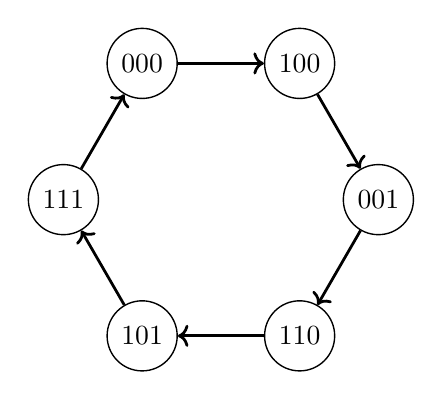
\begin{tikzpicture}
 \SetUpEdge[lw         = 1.0pt,
            color      = black,
            labelcolor = white]
  \GraphInit[vstyle=Normal] 
  \SetGraphUnit{3}
  \tikzset{VertexStyle/.append  style={fill}}
  %% 000, 100, 001, 110, 101, 111
  \Vertex[x=1,y=3.46]{000}
  \Vertex[x=3,y=3.46]{100}
  \Vertex[x=0,y=1.73]{111}
  \Vertex[x=4,y=1.73]{001}
  \Vertex[x=1,y=0]{101}
  \Vertex[x=3,y=0]{110}
  \tikzset{EdgeStyle/.style={->}}
  \Edge(000)(100)
  \Edge(100)(001)
  \Edge(001)(110)
  \Edge(110)(101)
  \Edge(101)(111)
  \Edge(111)(000)
\end{tikzpicture}

\section{State Table}
We shall start by writing the state table for the sequence
above. We shall be using D-Flip Flops for this exercise.
Since its a 3 bit counter, we need 3 D FlipFlops to
implement the sequence. Next, we create a truth table for
the D-Input of the flip-flops: 
\\\\
\begin{tabular}{a b c | d e f}
& Present state & & & Next State & &
\hline
A & B & C & A+ & B+ & C+ \\
0 & 0 & 0 & 1  & 0  & 0  \\
0 & 0 & 1 & 1  & 1  & 0  \\
0 & 1 & 0 & X  & X  & X  \\
0 & 1 & 1 & X  & X  & X  \\
1 & 0 & 0 & 0  & 0  & 1  \\
1 & 0 & 1 & 1  & 1  & 1  \\
1 & 1 & 0 & 1  & 0  & 1  \\
1 & 1 & 1 & 0  & 0  & 0  \\
\end{tabular} \\
We now have the truth table for next states. This table
can get Boolean expressions for logic.

\newpage    
\section{Karnaugh Map}
For a three-bit counter, the Karnaugh maps for the next state are as follows:
\\
A+
\begin{Karnaughvuit}
    \minterms{0,1,5,6}
    \maxterms{4,7}
    \indeterminats{2,3}
    \implicant{0}{2}{orange}
    \implicant{1}{5}{green}
    \implicant{2}{6}{green}
\end{Karnaughvuit}
\\
B+
\begin{Karnaughvuit}
    \minterms{1,5}
    \maxterms{0,4,6,7}
    \indeterminats{2,3}
    \implicant{1}{5}{green}
\end{Karnaughvuit}
\\
C+
\begin{Karnaughvuit}
    \minterms{4,5,6}
    \maxterms{0,1,7}
    \indeterminats{2,3}
    \implicant{4}{5}{purple}
    \implicant{2}{6}{green}
\end{Karnaughvuit}
\\
After minimization, we get the following equations:
\\$
A+ = A' + B'C + BC'
\\*
B+ = B'C
\\*
C+ = AB' + BC'$

\newpage
\section{Circuit}
It's time to draw the circuit in SimUAid using only D-Flip-Flops, NAND gates,
and inverters. Here is a logic circuit for the above truth tables. Note that
the S and R inputs are active low.
\\
\includegraphics[width=400px]{ckt}
\\
Note that if needed, the single inverter used could be substituted with a single NAND gate.



\end{document}
